\documentclass{article}
\usepackage{tikz}
\usepackage{xcolor}

\definecolor{myblue}{RGB}{40,110,160}
\definecolor{bggray}{RGB}{245,245,245}
\definecolor{gridgray}{RGB}{180,180,180}

\begin{document}

\begin{center}
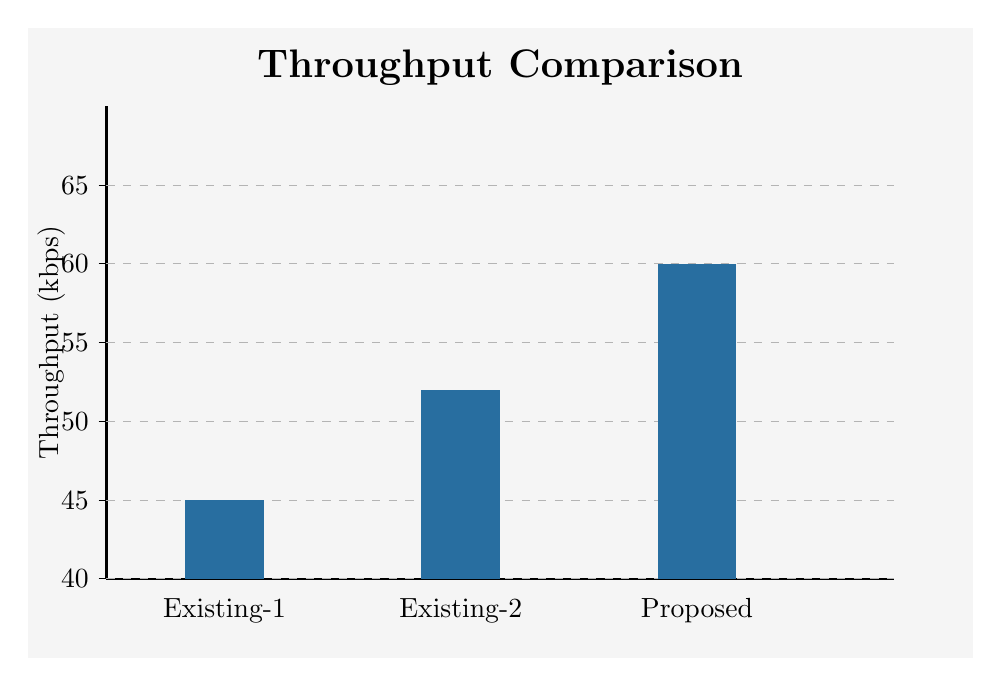
\begin{tikzpicture}

% Background
\fill[bggray] (0,0) rectangle (12,8);

% Axes
\draw[thick] (1,1) -- (1,7);
\draw[thick] (1,1) -- (11,1);

% Title
\node[font=\Large\bfseries] at (6,7.5) {Throughput Comparison};

% Labels
\node[rotate=90] at (0.3,4) {Throughput (kbps)};

% Y-axis ticks
\foreach \y/\val in {
1/40,
2/45,
3/50,
4/55,
5/60,
6/65
}{
\draw (0.9,\y) -- (1.1,\y);
\node[left] at (0.9,\y) {\val};
\draw[dashed, gridgray] (1,\y) -- (11,\y);
}

% Scale factor
\def\scale{0.2}

% Bars
\fill[myblue] (2,1) rectangle (3,{1+(45-40)*\scale});
\fill[myblue] (5,1) rectangle (6,{1+(52-40)*\scale});
\fill[myblue] (8,1) rectangle (9,{1+(60-40)*\scale});

% X labels
\node at (2.5,0.6) {Existing-1};
\node at (5.5,0.6) {Existing-2};
\node at (8.5,0.6) {Proposed};

\end{tikzpicture}
\end{center}

\end{document}